\begin{frame}
  \frametitle{2D Numerical results for \( hp \)-adaptivity}

  \begin{block}{The relative error}
    In energy-norm adaptivity, we define the relative error in percentage as:
    \begin{equation}
	 \tilde{e}_{\textrm{rel}}^{\textrm{energy}} \coloneqq \frac{\norm{u - u_{\calT_{c}}}_{\H}}{\norm{u}_{\H}} \cdot 100.
    \end{equation}
  \end{block}
  
  \begin{block}{Our Quantity of Interest (QoI)}
    For the GOA problems, we define our QoI as
    \begin{equation}
      l\left(\phi\right) = 
      \frac{1}{\abs{\Omega_{l}}} \scalaire{\mathds{1}_{\Omega_{l}}}{\phi}_{L^2(\Omega)}, 
      \quad \forall \phi \in \H,
    \end{equation}
    where:
    \begin{itemize}
      \item \( \abs{\Omega_{l}} \) defines the area or volume of \( \Omega_{l} \),
      \item \( \mathds{1}_{\Omega_{l}} \) is a function equal to one if \( x \in \Omega_{l} \), and zero otherwise.
    \end{itemize}
  \end{block}

\end{frame}

%\begin{frame}
%  \frametitle{2D Numerical results for $hp$-adaptivity}
%
%  \begin{block}{Singular Poisson example}
%    Find \(u\) satisfying:
%    \begin{alignat}{2}
%      - \Delta u & = \mathds{1}_{\Omega_{f}} && \quad \text{in } \Omega, \\
%      u          & = 0                       && \quad \text{on } \partial \Omega.
%    \end{alignat}
%  \end{block}
%
%  \begin{multicols}{2}
%   \textbf{Domain Definitions:}
%    \begin{itemize}
%      \item \(\Omega_{f} = \left(\frac{1}{4},\frac{1}{2}\right)^{2} \subset \Omega\), 
%      \item \(\Omega_{l} = \left(\frac{1}{2},\frac{3}{4}\right)^{2} \subset \Omega\),
%      \item \(a(\cdot ,\cdot) \coloneqq \scalar{\nabla \cdot}{\nabla \cdot}_{L^{2}(\Omega)}\).
%    \end{itemize}
% 
%    \begin{figure}
%       \centering
%  	 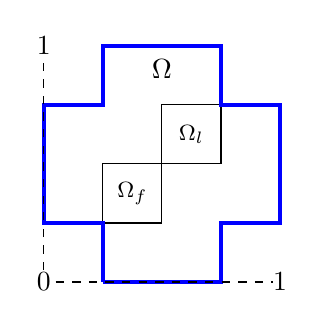
\begin{tikzpicture}[x=3cm,y=3cm]
        % Nodes for regions
        \node (n1) at (0.25,0) {};
        \node (n2) at (0.75,0) {};
        \node (n3) at (0.75,0.25) {};
        \node (n4) at (0.25,0.25) {};
        \node (n5) at (0.5,0.5) {};
        \node (n7) at (0.75,0.75) {};

        % Rectangles and labels
        \draw (n4) rectangle (n5) node[pos=0.5] {\footnotesize $\Omega_{f}$};
        \draw (n5) rectangle (n7) node[pos=0.5] {\footnotesize $\Omega_{l}$};

        % Boundary and labels
        \draw[line width=0.5mm, color=blue] (0.25,0) -- (0.75,0) -- (0.75,0.25) -- (1,0.25) -- (1,0.75) -- (0.75,0.75) -- (0.75,1) -- (0.25,1) -- (0.25,0.75) -- (0,0.75) -- (0,0.25) -- (0.25,0.25) -- (0.25,0);
        \node at (0.5,0.9) {$\Omega$};

        % Labels at specific coordinates
        \node at (0,0) {$0$};
        \node at (1,0) {$1$};
        \node at (0,1) {$1$};

        % Dashed lines connecting labels
        \draw[dashed] (0.05,0) -- (0.97,0);
        \draw[dashed] (0,0.05) -- (0,0.96);
      \end{tikzpicture}
%      \caption{Domain \\ $\Omega = \left(\left(0,1\right) \times \left(\frac{1}{4},\frac{3}{4}\right)\right) \cup \left(\left(\frac{1}{4},\frac{3}{4}\right) \times \left(0,1\right)\right)$.}
%    \end{figure}
%  \end{multicols}
%
%\end{frame}
%
%\begin{frame}
%	\frametitle{Singular Poisson example}
%	\begin{figure}[t!]
%   		\goasolutions{CrossGOA}{real}
%	\end{figure}
%\end{frame}
%
%\begin{frame}
%	\frametitle{Singular Poisson example}
%  	\plothpmeshes[]{CrossGOA}
%\end{frame}
%
%\begin{frame}
%\frametitle{Singular Poisson Example}
%\begin{figure}[t!]
%\centering
%\begin{tikzpicture}
\pgfplotsset{xmode=log, ymode=log} % Set log mode for both axes globally

\begin{axis}[
    name=mainerrorplot,
    xlabel={nDoFs (log scale)},
    ylabel={Relative error in \% (log scale)},
    ymode=log,
    xmode=log,
    width=0.9\plotwidth,
    height=0.9\plotheight,
    ylabel near ticks,
    xlabel near ticks,
    enlargelimits=true,
    legend style={
        draw=black,
        fill=white,
        legend cell align=left,
        at={(0.5,1.03)}, 
        anchor=south
    },
    legend columns=-1
]

% Plot for hp
\addplot+[line width=1pt] table[x expr=\thisrow{nr_dof}, y expr=\thisrow{Error}] {\FigurePath/CrossGOA/hp/order_1/outputs.txt}
    node[pos=0.85, pin={[pin edge=solid, pin distance=0.05cm]180:$hp$}] {}; % Adjusted pos from 0.9 to 0.85

% Plot for h with p=1
\addplot+[line width=1pt] table[x expr=\thisrow{nr_dof}, y expr=\thisrow{Error}] {\FigurePath/CrossGOA/h/order_1/outputs.txt}
    node[pos=0.9, pin={[pin edge=solid, pin distance=0.005cm]90:$h$ ($p=1$)}] {};

% Plot for h with p=2
\addplot+[line width=1pt] table[x expr=\thisrow{nr_dof}, y expr=\thisrow{Error}] {\FigurePath/CrossGOA/h/order_2/outputs.txt} 
    node[pos=1.010, pin={[pin edge=solid, pin distance=0.005cm]90:$h$ ($p=2$)}] {};

\end{axis}
\end{tikzpicture}
%\caption{Evolution of $e_{\textrm{rel}}^{\textrm{QoI}}$ in the adaptive process.}
%\end{figure}
%\end{frame}
